
\chapter{Interface Web}
\label{Logiciel}

Nous nous sommes penchés ensuite sur l'interface Homme/Machine. Dans une volonté de délivrer à l'utilisateur une interface agréable et lisible, nous avons décidé de proposer dans un premier temps une interface web.

\section{Analyse}
\label{sec:uml}

Dans un premier temps nous nous sommes penchés sur une  phase d'analyse.

Dans la phase d’analyse, nous cherchons d’abord à bien comprendre et à décrire de façon précise les besoins des utilisateurs ou des clients concernant cette interface. Que souhaitent-ils faire avec le logiciel ? Quelles fonctionnalités veulent-ils ? Pour quel usage ? Comment l’action devrait-elle fonctionner ? C’est ce qu’on appelle \og l’analyse des besoins\fg{}. Après validation de notre compréhension du besoin, nous imaginons la solution. C’est la partie analyse de la solution.

Dans la phase de conception, on apporte plus de détails à la solution et on cherche à clarifier des aspects techniques, tels que l’installation des différentes parties logicielles à installer sur du matériel. Pour réaliser ces deux phases dans un projet informatique, nous utilisons des méthodes, des conventions et des notations. UML fait partie des notations les plus utilisées aujourd’hui. Pour faciliter à nos clients d’obtenir la direction des drones on a créé une interface web qui répond à leur besoin.

\subsection{Uml}

Pour décrire au mieux ce besoin, nous avons commencé par réaliser un cas d'utilisation de l'interface (figure \ref{fig:use_case}).
\begin{figure}[!h]
  \centering
  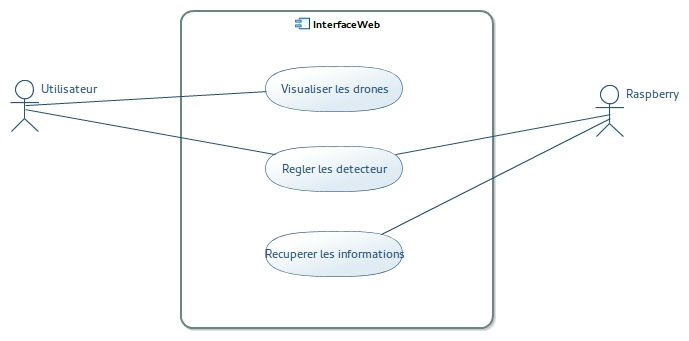
\includegraphics[width=\textwidth]{use_case}
  \caption{Cas d'utilisation de l'interface}
  \label{fig:use_case}
\end{figure}

\newpage
Ensuite, nous avons cherché à réaliser un diagramme de classe de notre interface. Pour cela nous avons défini 3 classes principales:

\begin{itemize}
\item index.php, qui réalise l'affichage dans un navigateur
\item serveur.py, qui récupère les données de chacun des radio-goniomètres
\item client.py, installé sur chaque radio-goniomètre il envoie les données des capteurs à travers un socket au serveur.
\end{itemize}

Le diagrammes de classe de la figure \ref{fig:class}, montre ce fonctionnement.

\begin{figure}[!h]
  \centering
  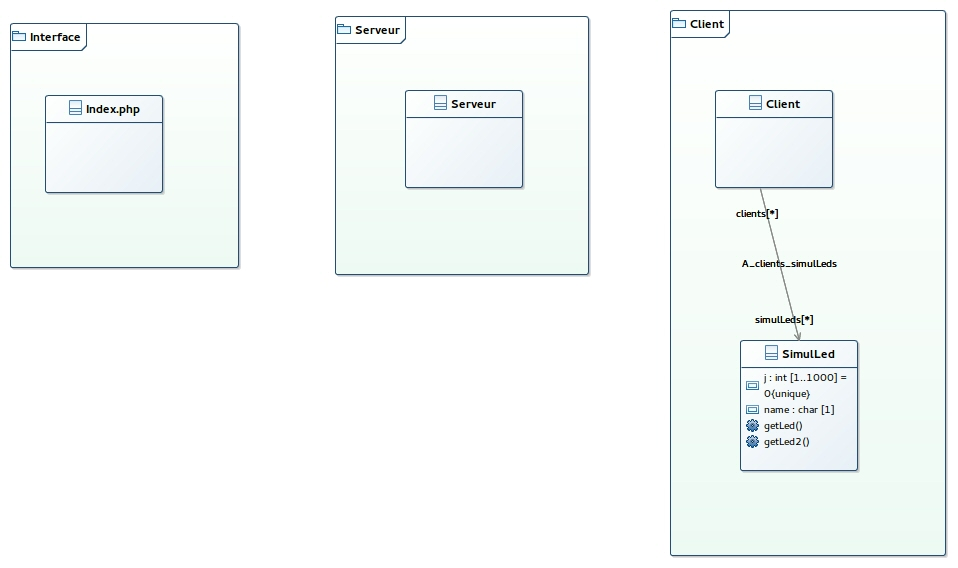
\includegraphics[width=\textwidth]{class_diagram}
  \caption{Diagramme de classe}
  \label{fig:class}
\end{figure}



\section{Conception}

\subsection{Client-Serveur}

Pour commencer nous avons cherché à donner une interface à nos \rpi pour communiquer avec l'ordinateur central, c'est l'interface Client/Serveur.
~\\

Cette interface a été codé en python. Nous avons choisi le python car c'est un langage souple et rapide. Nous avons réalisé la connection à l'aide d'un socket TCP/IP. De plus, le serveur se base sur du multi thread pour accepter plusieurs client. Le client se connecte donne, son identifiant puis sa communication est placé dans un thread. Ainsi, on a un serveur qui peut accepter une infinité de client.
~\\

Pour lancer le serveur il faut lancer le programme \textit{serveur.py} qui se met en écoute de client. Pour lancer le client il faut lancer le programme \textit{client.py}. Une illustration du terminal lors de l'exécution de ces commandes est donnée ci-dessous.
~\\

\begin{minipage}[h]{0.45\linewidth}

\begin{lstlisting}
./serveur.py
Serveur pret, en attente de requetes ...
Client RP1 connecte, adresse IP 127.0.0.1, port 51632.
RP1> led21
donc la direction 200
[...]
Client RP1 deconnecte.
[...]
Fin du serveur
\end{lstlisting}  
\end{minipage}\hfill
\begin{minipage}[h]{0.45\linewidth}
  
\begin{lstlisting}
./client.py
Connexion etablie avec le serveur.
Vous etes connecte. Envoyez vos messages.
la led allume: led21
[...]
Connexion interrompue.
\end{lstlisting}

\end{minipage}

~\\

On peut constater que la seule donnée que le \rpi envoie en continue est le numéro de la led qui s'est allumé. En effet, le modèle du Montréal 3v2 affiche le gisement sur un cadrant de 36 led. Dans notre solution nous avons décidé de garder ce cadrant et de placer le \rpi en parallèle du circuit pour détecter laquelle led s'est allumé. De plus, nous avons décidé de réaliser la conversion led/gisement au niveau du serveur pour des questions de modularités. 

~\\

Une foi les données reçut par le serveur, celui-ci les écrit dans un fichier qui s'appelle \textit{position}.



\subsection{Web}

Ensuite, nous nous sommes penché sur notre page web. Cette page web doit permettre à notre utilisateur de visualiser en temps réel la position du drone dans notre maillage. Pour cela nous avons fait le choix d'utiliser des solutions dynamiques tel que PHP, Javascript et JQuery.
~\\

Pour nous faciliter dans la réalisation du schéma modélisant notre treillis, nous avons choisi SVG. En effet, SVG nous permet de réaliser notre schéma de manière vectorielle. C'est-à-dire que l'on peut donner avec précision la position des capteurs ainsi que de leur droite de détection, mais surtout on peut rendre cela dynamique.
~\\

Le script ouvre le fichier \textit{position} qui a été précédemment rempli, et ajoute les points qui sont inscrit dans le fichier avec leur droite de détection. Mais cela ne suffit pas. En effet, si l'on s'arrête là on n'a qu'une position visible par un être humain il reste encore à la positionner. Pour cela nous utiliserons la triangulation (voir à la page \ref{sec:trian}).
~\\

Enfin, nous affichons de manière classé l'ensemble des \rpi qui été présent dans le fichier position à la droite de l'écran.




\subsection{Triangulation}
\label{sec:trian}
Les différents radiogoniomètres nous donnant un gisement de la détection, nous pouvons donc
réaliser une triangulation de la position du drone lorsqu’un nombre suffisant d’antenne détecte le
drone. Bien qu’une première estimation de la position peut-être obtenu à partir de deux drones,
nous considérons que le drone doit être détecté par au moins quatre senseurs pour que la position
soit acceptable.
~\\

Cependant, avant de pouvoir réaliser toute triangulation, l’acquisition des points d’intersection entre
les droites de détection issue du gisement fourni par les différents radiogoniomètres est nécessaire.
Pour se faire, à partir des angles, nous formulons une équation de droite plan, passant par les
radiogoniomètres respectifs, et tentons de trouver une solution à chaque système composé de deux
droites.
~\\

\begin{wrapfigure}{r}{0.5\textwidth}

  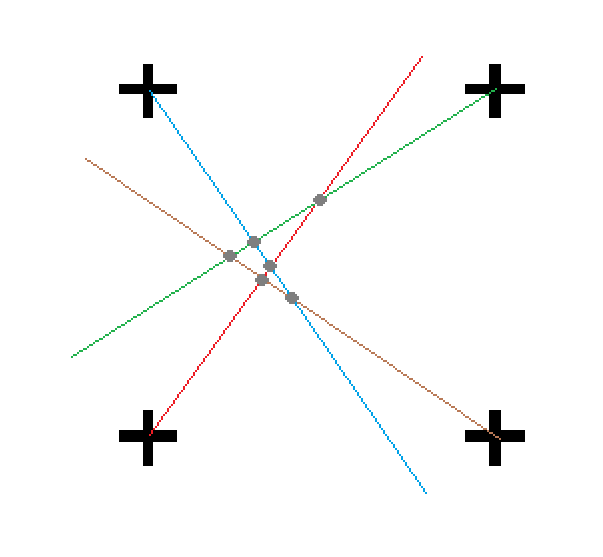
\includegraphics[width=0.5\textwidth]{triangulation1}
  \caption{triangulation}
\end{wrapfigure}

  Suite à la résolution de ces différents systèmes, nous
obtenons une liste de différentes solutions, solutions ici
schématisé avec des points de couleur grise. Nous observons
que, du fait de la portée de détection, ainsi que la géométrie
de notre treillis, certains points sont incohérents ou très
imprécis.

~\\
Notre première approche fut donc de positionner le drone à
la moyenne de l’ensemble des positions solutions d’un des
systèmes précédent. Cependant, après simulation, il s’est
avéré que, de par l’imprécision relative des
radiogoniomètres (les angles sont donnée à 5\up{o} près), la moyenne de donnait qu’une idée toute relative de la position du drone et souvent loin de la vérité, et
cela à cause d’intersections multiples entre les droites de détection.
Pour corriger cela nous avons fait le choix d’utiliser la médiane afin de supprimer tous les résultats
incohérents. A partir de la médiane des résultats, nous appliquons un gabarit circulaire et retenons
tous les points d’intersection compris dans ce gabarit. Une moyenne est alors appliquée à l’ensemble
de ces résultats nous permettant d’obtenir un résultat plus cohérent et moins sensible aux erreurs.


~\\
\newpage
Au final, nous obtenons la page web suivante:

\begin{figure}[!h]
  \centering
  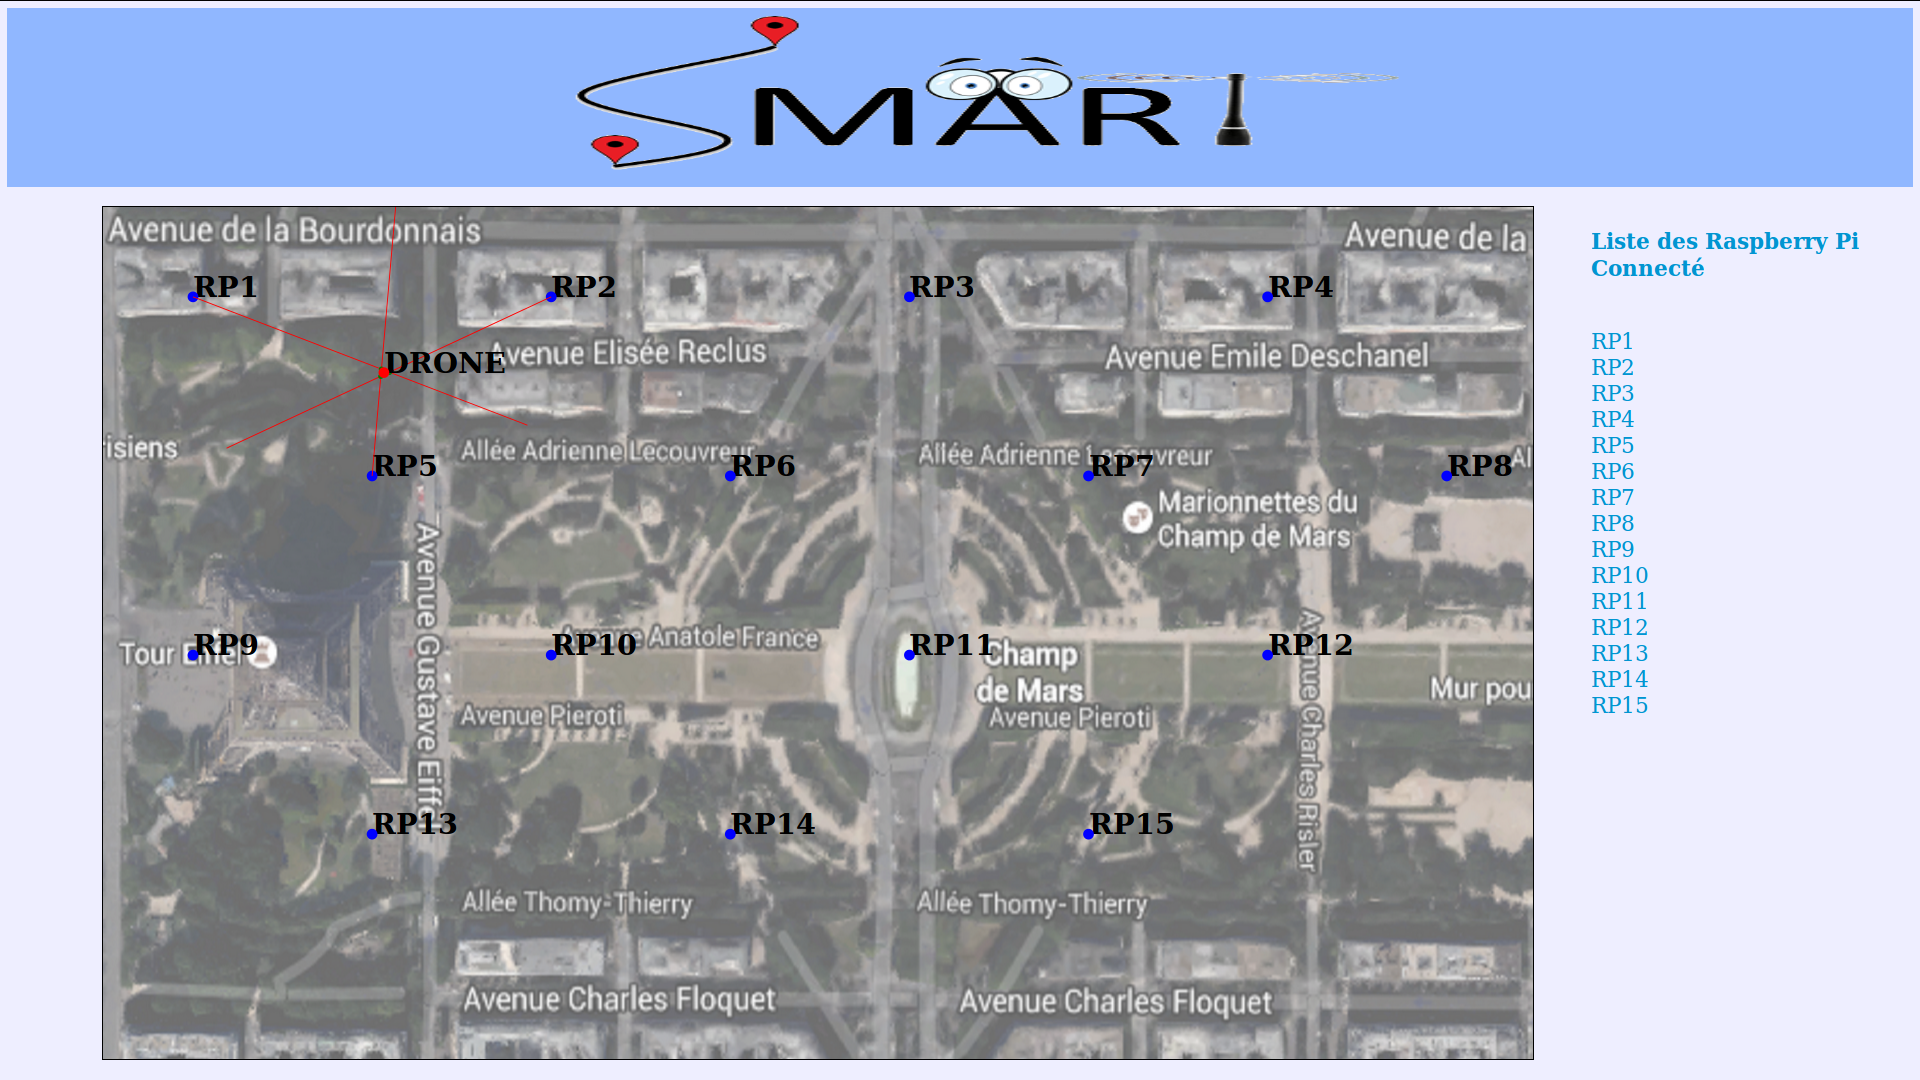
\includegraphics[width=\textwidth]{interface}
  \caption{Interface Web}
  \label{fig:interface}
\end{figure}





%%% Local Variables: 
%%% mode: latex
%%% TeX-master: "../rapport"
%%% End: 
